% !TEX root = 1_power_supply.tex
\documentclass[1_power_supply.tex]{subfiles}
\graphicspath{{../figures/}}
\begin{document}

\section{DC-DCコンバータ}

\subsection{目的}

太陽電池から得られる直流の電圧,電流を増幅するためにDC-DCコンバータ農地,チュックコンバータを用いる.本実験では,チュックコンバータのスイッチ制御を変化させたときの電力利得を調べる.

\subsection{原理}

\subsection{方法}

\begin{figure}[htbp]
	\begin{center}
		\scalebox{0.1}{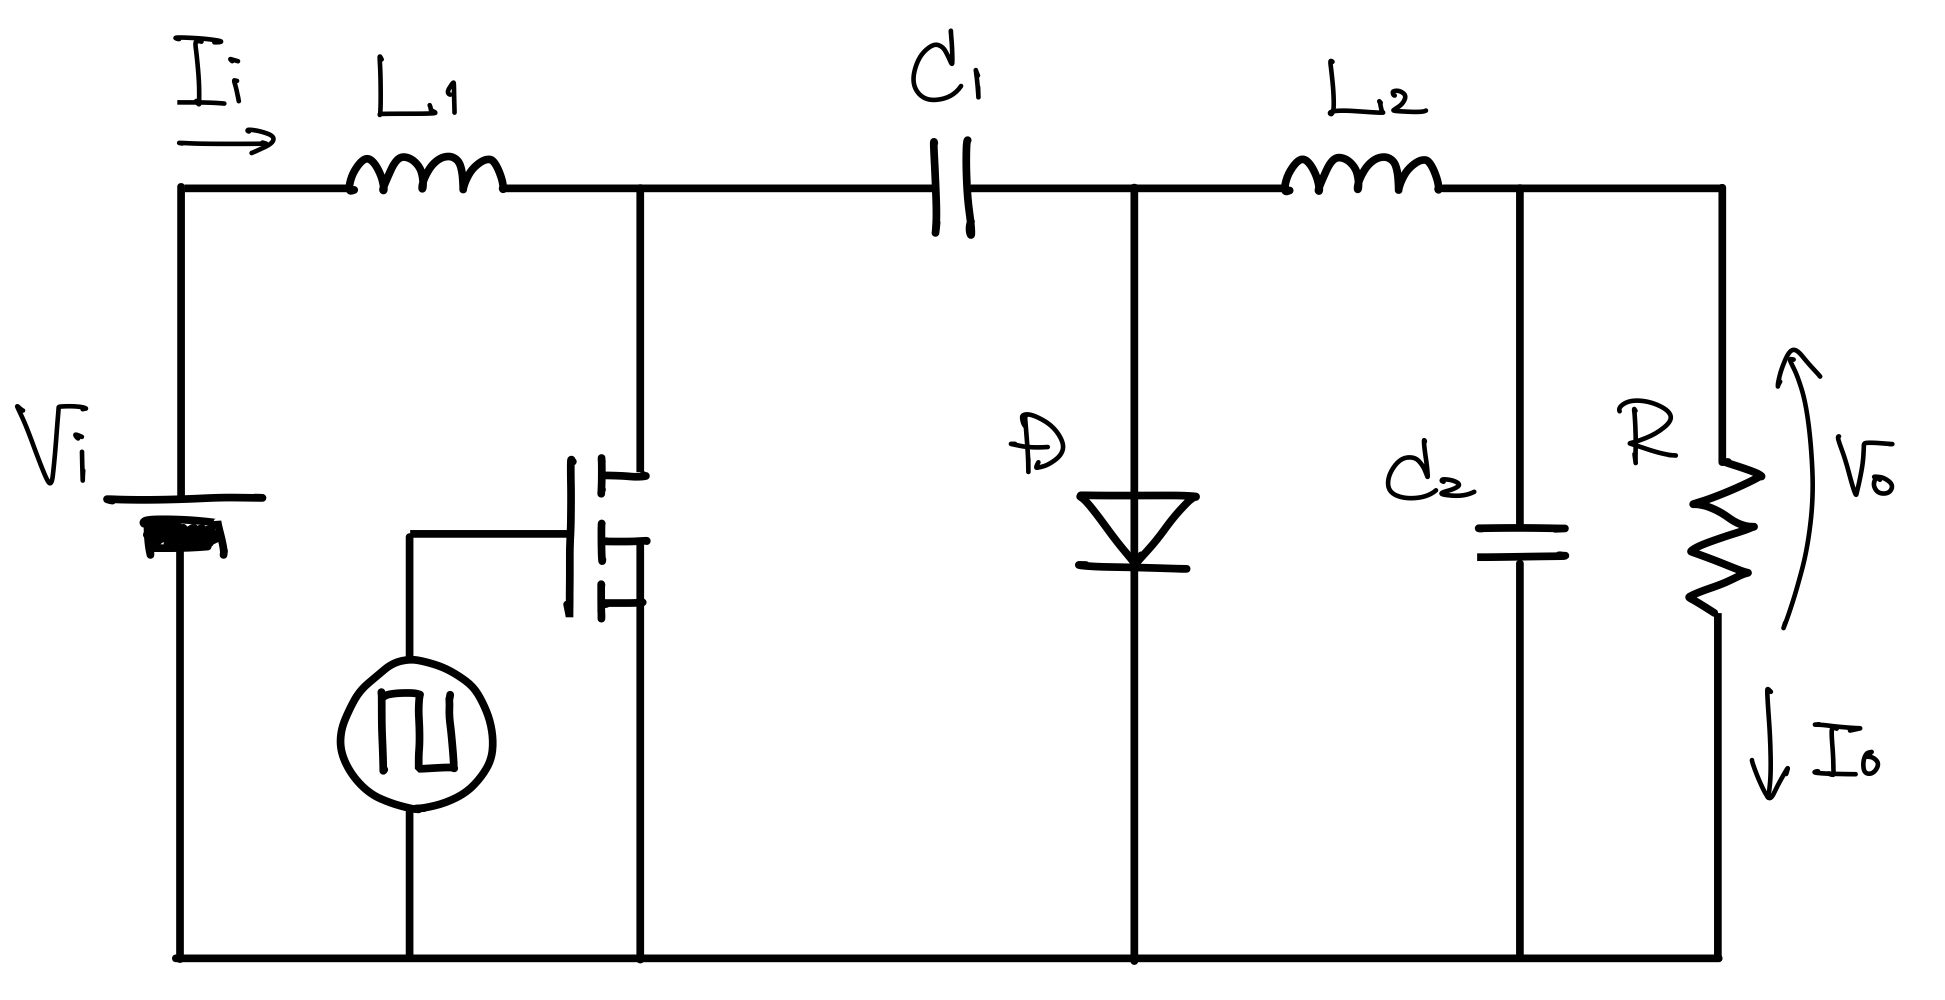
\includegraphics{1_4.png}}
		\caption{測定対象の回路}\label{fig:1_4}
	\end{center}
\end{figure}

\subsection{使用器具}

\subsection{結果}

\begin{figure}[htbp]
	\begin{minipage}{0.45\columnwidth}
		\centering
		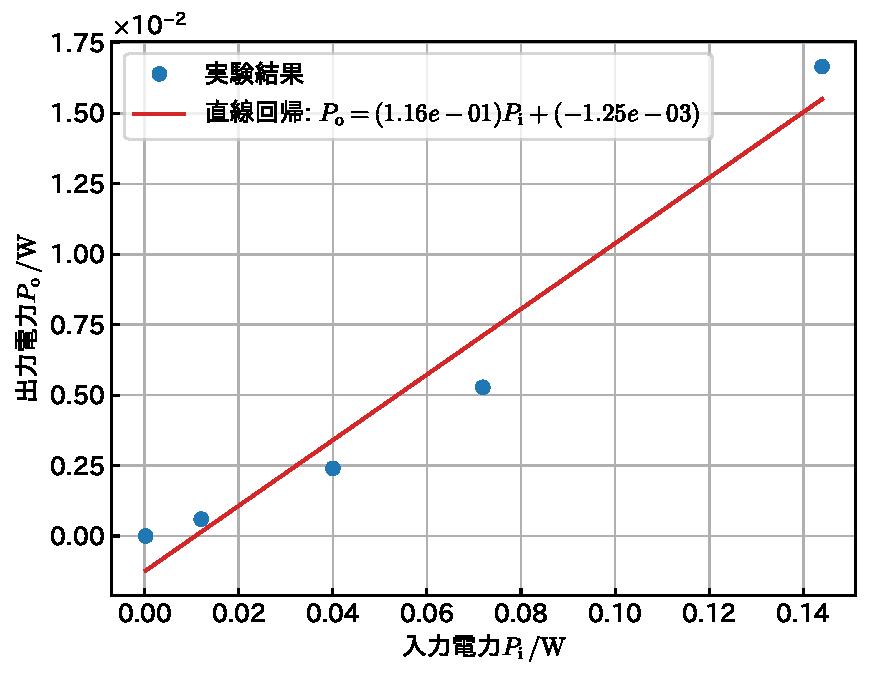
\includegraphics[width=0.8\columnwidth]{2_10p.pdf}
		\caption{}\label{fig:2_10p}
	\end{minipage}
	\begin{minipage}{0.45\columnwidth}
		\centering
		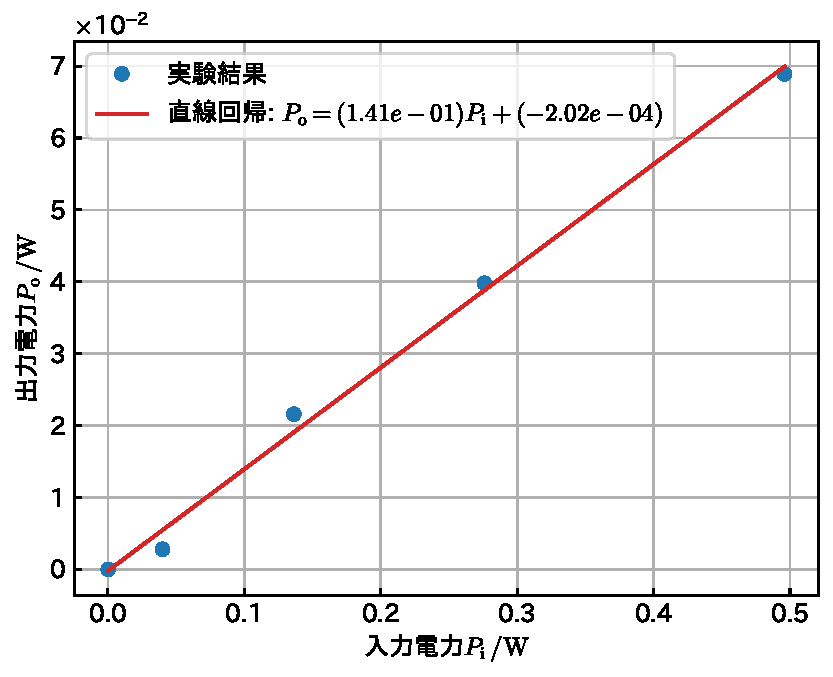
\includegraphics[width=0.8\columnwidth]{2_25p.pdf}
		\caption{}\label{fig:2_25p}
	\end{minipage}

	\vspace{1mm}
	\begin{minipage}{0.45\columnwidth}
		\centering
		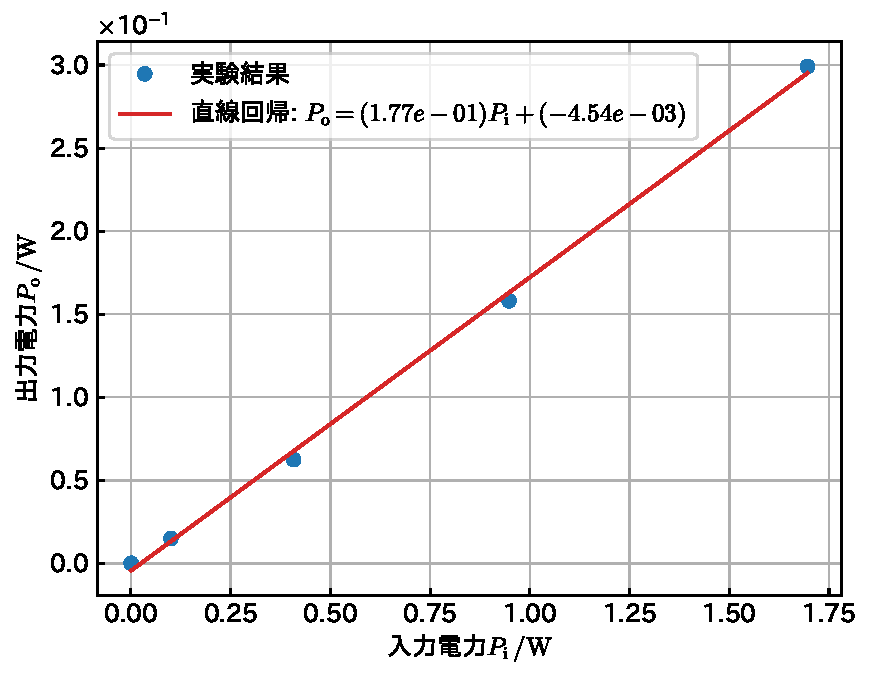
\includegraphics[width=0.8\columnwidth]{2_40p.pdf}
		\caption{}\label{fig:2_40p}
	\end{minipage}
	\begin{minipage}{0.45\columnwidth}
		\centering
		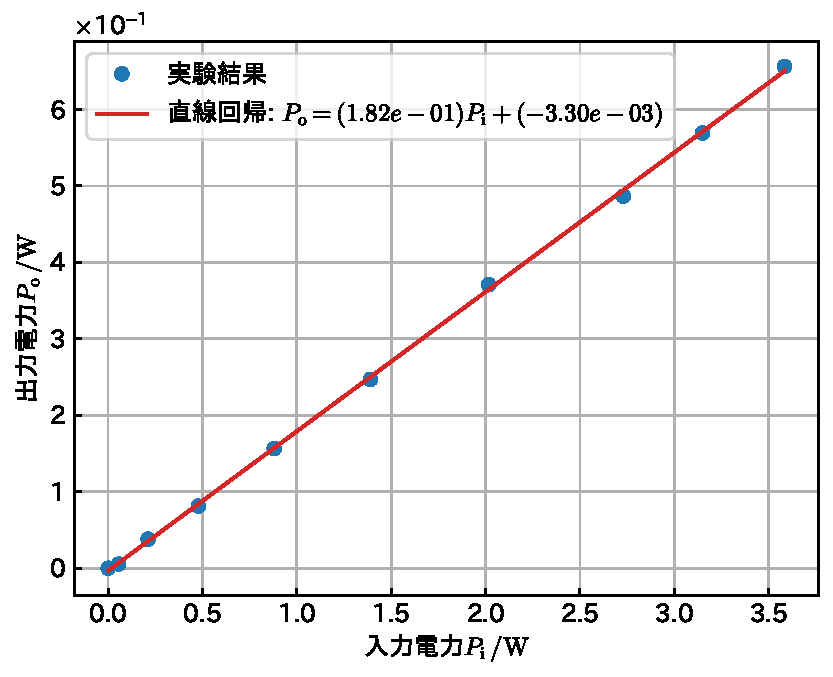
\includegraphics[width=0.8\columnwidth]{2_50p.pdf}
		\caption{}\label{fig:2_50p}
	\end{minipage}

	\vspace{1mm}
	\begin{minipage}{0.45\columnwidth}
		\centering
		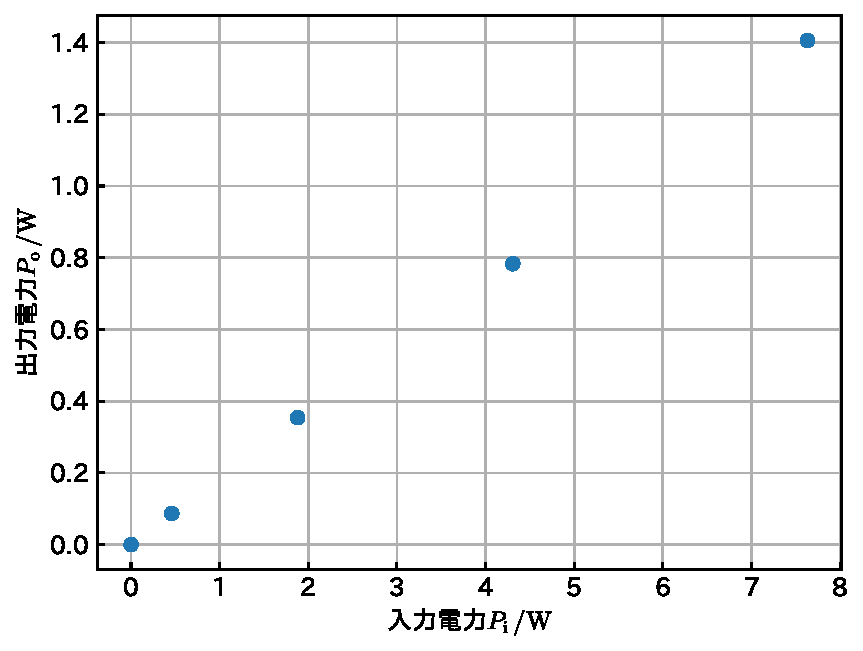
\includegraphics[width=0.8\columnwidth]{2_60p.pdf}
		\caption{}\label{fig:2_60p}
	\end{minipage}
	\begin{minipage}{0.45\columnwidth}
		\centering
		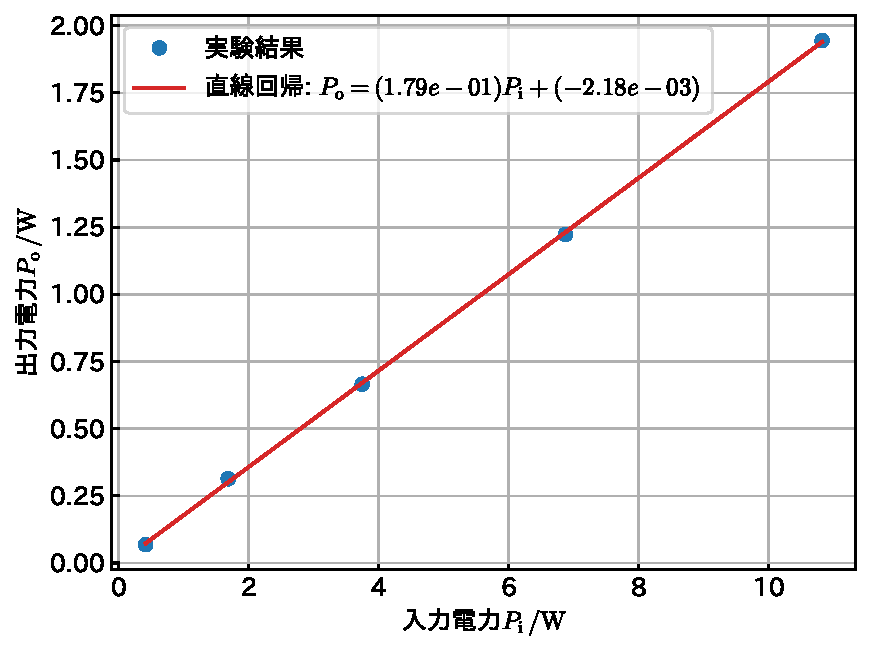
\includegraphics[width=0.8\columnwidth]{2_75p.pdf}
		\caption{}\label{fig:2_70p}
	\end{minipage}

	\vspace{1mm}
	\begin{minipage}{0.45\columnwidth}
		\centering
		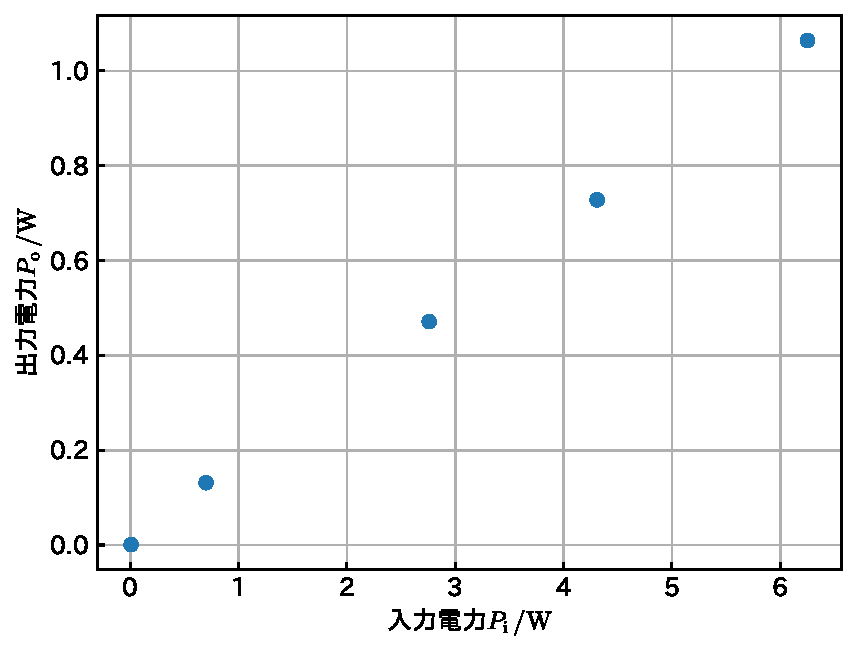
\includegraphics[width=0.8\columnwidth]{2_80p.pdf}
		\caption{}\label{fig:2_80p}
	\end{minipage}
	\begin{minipage}{0.45\columnwidth}
	\end{minipage}
\end{figure}

\subsection{考察}
